\section{System design}
\begin{figure}[t]
	\centering
	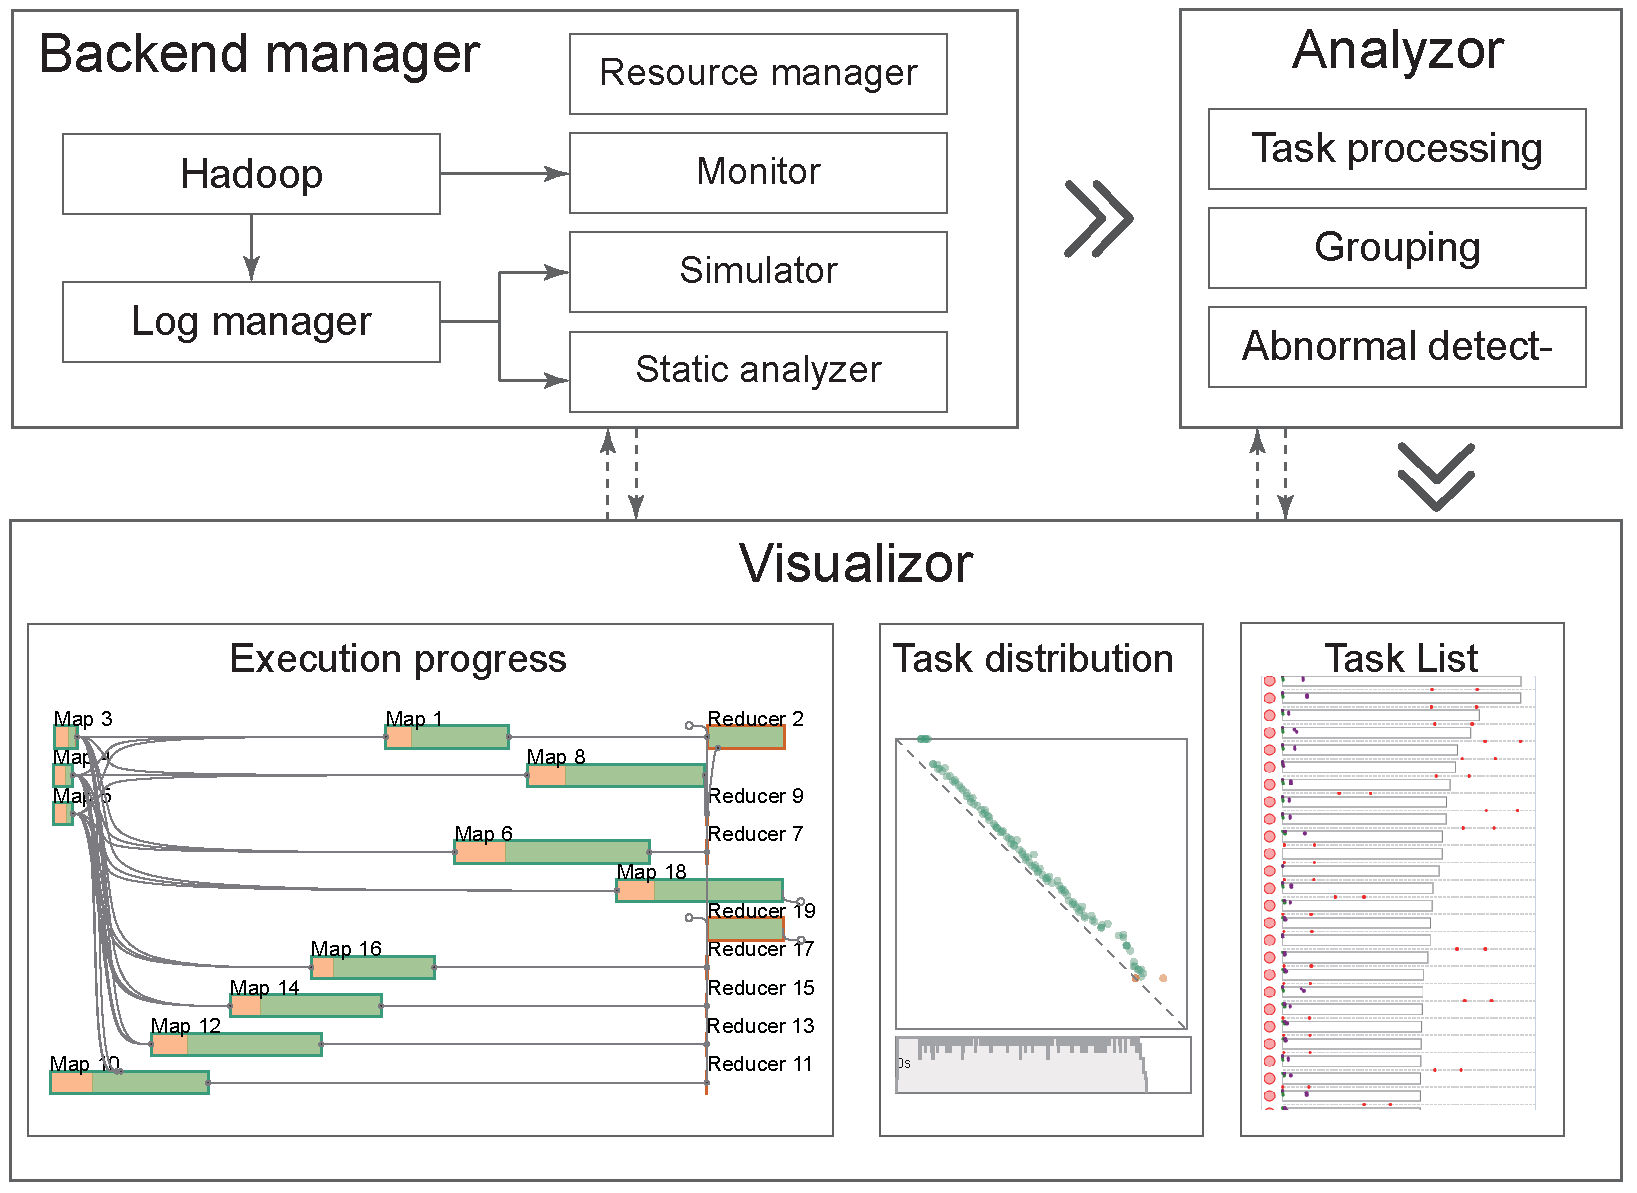
\includegraphics[width=0.45\textwidth]{figures/system/sysdesign.pdf}
	\vspace{-3mm}
	\caption{$\DQV$ system consists of three major components: backend manager, analyzer and visualizer.}
	\label{fig:sysdesign}
	\vspace{-3mm}
\end{figure}
We use build $\DQV$ based on Hadoop2.0 with \textbf{Hive} as query optimizer and \textbf{Tez} as the executor. As shown by Figure~\ref{fig:sysdesign}, $\DQV$ consists of three modules: backend manager, analyzer, and visualizer. 


The \textbf{Backend Manager} module performs the log processing and data fusion. Two categories of data are collected and fused: the execution data and the system performance data.
When collecting the execution data from Hadoop system, the Log Manager cleans and preprocesses the log files, extracts the important metrics and saves them as the local files.
Log analyzer directly takes these files as input and processes them as structured data for future processing.
Monitor module segments the data at the specific time range and output them with a given rate.
The simulator simulates the execution progress, allowing users to adjust the running speed and explore the dynamic query process.
Moreover, Resource Manager collect the system performance metrics and output them to the next processing stage.


The \textbf{Analyzer} fuses the execution data and system performance data by timestamps. The tasks will be grouped according to the vertex of the execution plan. The dataflow dependencies are recorded in this step. Moreover, Analyzor also performs the anomaly detection for the tasks in a group to enable the in-depth analysis.


The \textbf{Visaulizor} module integrates coordinated views to support interactive exploration of query execution results and reasoning about the query behavior at multiple levels. The Execution Overview demonstrates the execution process at the vertex level. An algorithm for the temporal DAG is proposed to visualize the structure and procedure simultaneously. The task group view consists of two components: 1) task overview visualizes the temporal information and data dependencies of tasks executed on the same machine; 2) metrics component shows the corresponding machine performance metrics. The task list view provides more detailed information at the operator level, enabling the users to understand and compare the time usage of tasks. 

